\section{Problem Formulation}\label{sec:problem}
As shown in Fig.~\ref{fig:allvits}, most modern vision transformers exhibit artifacts in the attention maps.
The unsupervised DINO backbone~\new{\citep{caron2021emerging}}\old{\cite{caron2021emerging}} has been previously praised for the quality of local features and interpretability of attention maps.
Surprisingly, the outputs of the subsequent DINOv2 models have been shown to hold good local information but exhibit undesirable artifacts in attention maps.
In this section, we propose to study \textit{why} and \textit{when} these artifacts appear.
While this work focuses on alleviating artefacts in all vision transformers, we focus our analysis on DINOv2.

\subsection{Artifacts in the local features of DINOv2}
\label{subsec:artifacts}

\paragraph{Artifacts are high-norm outlier tokens.}
We want to find a quantitative way of characterizing\old{the} artefacts that appear in the local features.
We observe that an important difference between ``artifact'' patches and other patches is the norm of their token embedding at the output of the model.
In Fig.~\ref{fig:norms_hist} (left), we \old{show}\new{compare} the norm of local features for a DINO and DINOv2 model \old{for}\new{given} a reference image.
We clearly see that the norm of artifact patches is much higher than the norm of other patches.
We also plot the distribution of feature norms over a small dataset of images in Fig.~\ref{fig:norms_hist} (right), \new{which is clearly bimodal}, allowing us to choose a simple criterion for the rest of this section: tokens with norm higher than 150 will be considered as ``high-norm'' tokens, and we will study their properties relative to regular tokens. 
This hand-picked cutoff value can vary across models. 
In the rest of this work, we use ``high-norm'' and ``outlier'' interchangeably.

\paragraph{Outliers appear during the training of \old{larger}\new{large} models.}
We make several additional observations about the conditions in which these outlier patches appear \old{in}\new{during} the training of DINOv2.
This analysis is illustrated in Fig.~\ref{fig:factors_choice}.
First, these high-norm patches seem to differentiate themselves from other patches around layer 15 of this 40-layer ViT (Fig.~\ref{fig:norm_hist_by_layer}).
Second, when looking at the distribution of norms along training of DINOv2, we see that these outliers only appear after one third of training (Fig.~\ref{fig:norm_hist_by_iter}).
Finally, when analyzing more closely models of different size (Tiny, Small, Base, Large, Huge and giant), we see that only the \old{larger}\new{three largest} models \old{suffer from}\new{exhibit} outliers (Fig.~\ref{fig:norm_hist_by_model}).

\begin{figure}[t]
  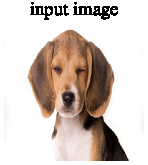
\includegraphics{resources/figure_3_1.pdf} 
  
\includegraphics{resources/figure_3_2.pdf} 
  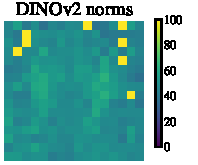
\includegraphics{resources/figure_3_3.pdf} 
  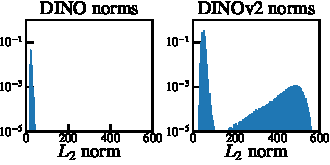
\includegraphics{resources/figure_3_4.pdf} 
  \caption{
    Comparison of local feature norms for DINO ViT-B/16 and DINOv2 ViT-g/14. 
    We observe that DINOv2 has a few outlier patches, whereas DINO does not present these artifacts. 
    For DINOv2, although most patch tokens have a norm between 0 and 100, a small proportion of tokens have a very high norm. 
    We measure the proportion of tokens with norm larger than 150 at 2.37\%.
  }  
  \label{fig:norms_hist}
\end{figure}


\paragraph{High-norm tokens appear where patch information is redundant.} 
To verify this, we measure the cosine similarity between \old{the} high-norm tokens and their 4 neighbors right after the patch embedding layer (at the beginning of the vision transformer). 
We illustrate the density plot in Fig. \ref{fig:outlier_cos_sims}.
We observe that \old{the} high-norm tokens appear on patches that \old{have a \old{very} high similarity with their neighbors. \old{, compared to other patches. }}\new{are very similar to their neighbors.}
This suggests that these patches \old{\old{are}\new{share} redundant \old{to}\new{information with} their neighbors, }\new{contrain redundant information} and that the model could
\old{\old{discard their information without losing much information}\new{discard them without hurting the performance on future downstream tasks}}\new{discard their information without hurting the quality of the image representation}.
This matches qualitative observations (see Fig.~\ref{fig:allvits}) that they often appear in uniform, background areas.

\begin{figure}[t]
  \centering
  \subcaptionbox{Norms along layers.\label{fig:norm_hist_by_layer}}{
    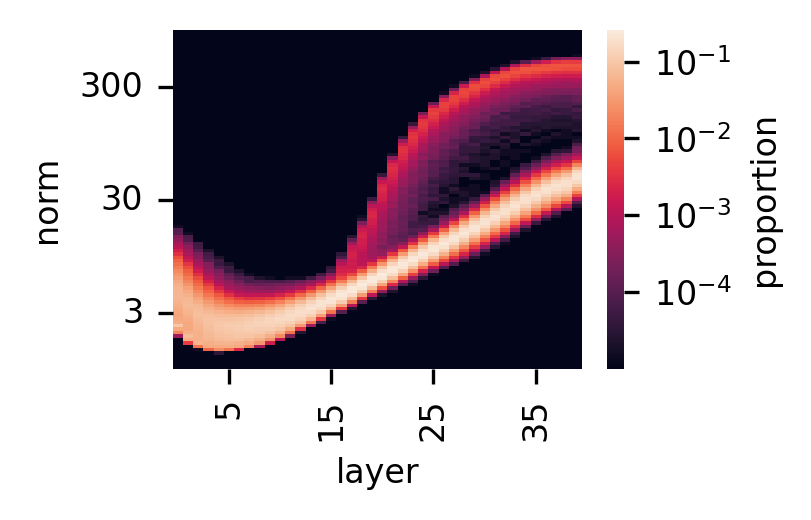
\includegraphics[width=0.31\linewidth]{resources/230802_norm_histogram_by_layer.png}
  }
  \subcaptionbox{Norms along iterations.\label{fig:norm_hist_by_iter}}{
    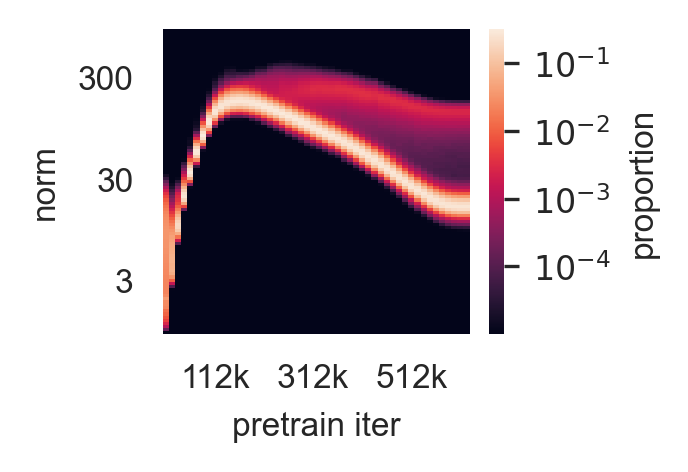
\includegraphics[width=0.31\linewidth]{resources/norm_distrib_vs_pretrain_iter.png}
  }
  \subcaptionbox{Norms across model size.\label{fig:norm_hist_by_model}}{
    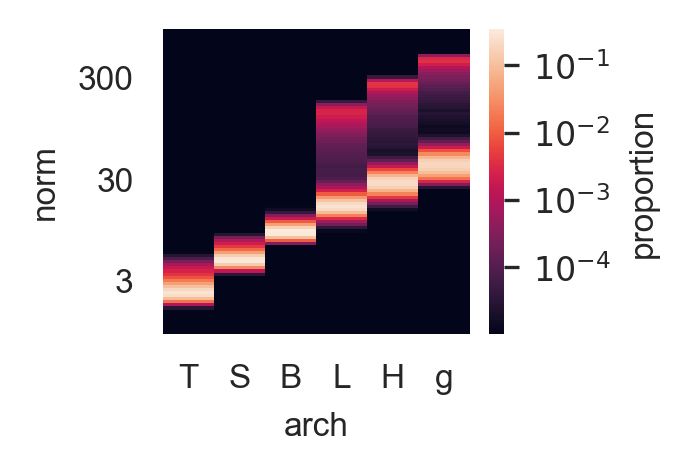
\includegraphics[width=0.31\linewidth]{resources/norm_distrib_vs_model_size.png}
  }
  \caption{
    Illustration of several properties of outlier tokens in the 40-layer DINOv2 ViT-g model.
    \textbf{(a)}: Distribution of output token norms along layers.
    \textbf{(b)}: Distribution of norms along training iterations.
    \textbf{(c)}: Distribution of norms for different model sizes. The outliers appear around the middle of the model during training; they appear with models larger than and including ViT-Large.
  }
  \label{fig:factors_choice}
\end{figure}


\paragraph{High-norm tokens hold little local information.}
In order to better understand the nature of these tokens, we propose to probe the patch embeddings for different types of information. 
For that we consider two different tasks: position prediction and pixel reconstruction. 
For each of these tasks, we \old{will} train a linear model on top of the patch embeddings, and measure the performance of this model. 
We \old{will} compare the performance \old{of this model}\new{achieved with}\old{on the} high-norm tokens and \old{on the}\new{with} other tokens, to see if \old{the} high-norm tokens contain different information than \old{the other}\new{``normal''} tokens.

\begin{itemize}
  \item \textbf{Position prediction.}
  We train a linear model to predict the position of each patch token in the image, and measure its accuracy. We note that this position information was injected in the tokens before the first ViT layer in the form of absolute position embeddings.
  We observe that high-norm tokens have \old{a} much lower accuracy than the other tokens (Fig.~\ref{tab:logreg_weird_patches_local}), suggesting
  they contain less information about their position in the image.\old{ than other tokens.}
  \item \textbf{Pixel reconstruction.}
  We train a linear model to predict the pixel values of the image from the patch embeddings, and measure the accuracy of this model.
  We observe \new{again} that \old{the} high-norm tokens \new{achieve}\old{have a} much lower accuracy than \old{the} other tokens (Fig.~\ref{tab:logreg_weird_patches_local}).
  This suggests that \old{the} high-norm tokens contain less information to reconstruct the image than the others.
\end{itemize}

\begin{figure}[t]
  \centering
  \subcaptionbox{Cosine similarity to neighbors.\label{fig:outlier_cos_sims}}{
    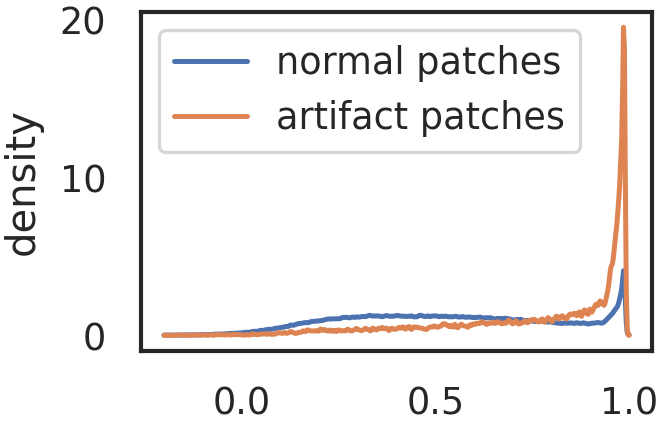
\includegraphics[width=0.3\linewidth]{resources/230802_kde_cossim_neighbors_2.png}
  }
  \hfill
  \subcaptionbox{Linear probing for local information.\label{tab:logreg_weird_patches_local}}{
    \begin{tabular}{@{} l c cc c c @{}}
      \toprule
              && \multicolumn{2}{c}{position prediction} && reconstruction\\
      \cmidrule{3-4} \cmidrule{6-6}
              && top-1 acc      & avg. distance $\downarrow$ && L2 error $\downarrow$\\
      \midrule
      normal  && \textbf{41.7}  & \textbf{0.79} && \textbf{18.38} \\
      outlier && 22.8           & 5.09          && 25.23 \\
      \bottomrule
    \end{tabular}
  }
  \caption{
    \textbf{(a)}: Distribution of cosine similarity between input patches and their 4 neighbors.
    We plot separately artifact patches (norm of the \emph{output token} over 150) and normal patches.
    \textbf{(b)}: Local information probing on normal and outlier patch tokens. 
    We train two models: one for predicting position, and one for reconstructing the input patch.
    Outlier tokens have much lower scores than the other tokens, suggesting they are storing less local patch information.
  }
\end{figure}


\paragraph{Artifacts hold global information.}
In order to evaluate how much global information is gathered in the high-norm tokens, we propose to evaluate them on standard image representation learning benchmarks.
For each image in a classification dataset, we forward it through DINOv2-g and extract the patch embeddings.
From those, we choose a single token at random, either high-norm or normal.
This token is then considered as the image representation.
We then train a logistic regression \new{classifier} to predict the image class from this representation, and measure the accuracy. \old{of this model.}
We observe that the high-norm tokens have a much higher accuracy than the other tokens (Table~\ref{tab:logreg_weird_patches_image_classif}).
This suggests that \old{the} outlier tokens contain more global information than \old{the} other patch tokens.

\begin{table}[t]
  \centering
  \begin{tabular}{@{} l *{14}{c@{\hspace{4pt}}} @{}}
    \toprule
    & IN1k & P205 & Airc. & CF10 & CF100 & CUB & Cal101 & Cars & DTD & Flow. & Food & Pets & SUN & VOC \\
    \midrule
    \texttt{[CLS]} & \textbf{86.0} & \textbf{66.4} & \textbf{87.3} & \textbf{99.4} & \textbf{94.5} & \textbf{91.3} & \underline{96.9} & \textbf{91.5} & \textbf{85.2} & \textbf{99.7} & \textbf{94.7} & \textbf{96.9} & \textbf{78.6} & \underline{89.1} \\
    normal & 65.8 & 53.1 & 17.1 & 97.1 & 81.3 & 18.6 & 73.2 & 10.8 & 63.1 & 59.5 & 74.2 & 47.8 & 37.7 & 70.8 \\
    outlier & \underline{69.0} & \underline{55.1} & \underline{79.1} & \underline{99.3} & \underline{93.7} & \underline{84.9} & \textbf{97.6} & \underline{85.2} & \underline{84.9} & \underline{99.6} & \underline{93.5} & \underline{94.1} & \underline{78.5} & \textbf{89.7} \\
    \bottomrule
  \end{tabular}
  \caption{
    Image classification via linear probing on normal and outlier patch tokens. 
    We also report the accuracy of classifiers learnt on the class token.
    We see that outlier tokens have a much higher accuracy than regular ones, suggesting they are effectively storing global image information.
  }
  \vspace{-1em}
  \label{tab:logreg_weird_patches_image_classif}
\end{table}



\subsection{Hypothesis and remediation}
\label{sec:hypothesis}
Having made these observations, we make the following hypothesis: \emph{large}, \emph{sufficiently trained} models learn to recognize \emph{redundant} tokens, and to use them as places to \emph{store}, \emph{process} and \emph{retrieve} global information.
Furthermore, we posit that while this behavior is not bad in itself, the fact that it happens inside the patch tokens is undesirable.
Indeed, it leads the model to discard local patch information (Tab.~\ref{tab:logreg_weird_patches_local}), possibly incurring decreased performance on dense prediction tasks. %

We therefore propose a simple \old{and natural} fix to this issue: we explicitly add new tokens to the sequence, that the model can learn to use as registers.
We add these tokens after the patch embedding layer, with a learnable value, similarly to the \texttt{[CLS]} token.
At the end of the vision transformer, these tokens are discarded, and the \texttt{[CLS]} token and patch tokens are used as image representations, as usual.
This\old{is a} mechanism \old{that} was \new{first} proposed in Memory Transformers \citep{burtsev2020memory}, improving translation tasks in NLP. \new{Interestingly, we show here that this mechanism admits a natural justification for vision transformers, fixing an interpretability and performance issue that was present otherwise. }
\old{, but was never \new{studied 
for large-scale vision transformers.}\old{or used with Vision Transformers.}}


We note that we have not been able to fully determine which aspects of the training led to the appearance of artifacts in different models. The pretraining paradigm seems to play a role, as OpenCLIP and DeiT-III exhibit outliers both at size B and L (Fig. \ref{fig:allvits}). However, the model size and training length also play important parts, as observed in Fig. \ref{fig:factors_choice}.


\begin{figure}[t]
  \centering
  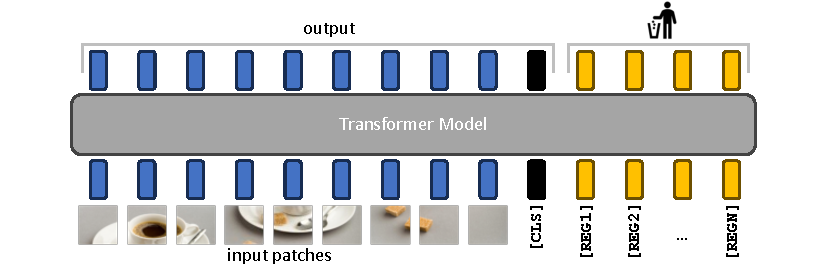
\includegraphics{resources/model.pdf} 
  \caption{
    Illustration of the proposed remediation and resulting model.
    We add $N$ additional learnable input tokens (depicted in yellow), that the model can use as \emph{registers}.
    At the output of the model, only the patch tokens and \texttt{[CLS]} tokens are used, both during training and inference.
  }  
  \vspace{-1em}
  \label{fig:model}
\end{figure}
